%! TeX program = lualatex
\documentclass[../main.tex]{subfiles}

\begin{document}

\section{Week 2 practice problems}

\begin{exercise}
  For each recurrence below, calculate \(u_{1}, u_{2}, u_{3}\).
  \begin{enumerate}
    \item \(u_{0} = 3\) and \(u_{t} = u_{t-1}^{2}\) for integers \(t \ge 1\)

      \begin{solution}
        \begin{align*}
          u_{0} &= 3, &\text{(given)} \\
          u_{1} &= u_{0}^{2} = 3^{2} = 9, \\
          u_{2} &= u_{1}^{2} = 9^{2} = 81,\\
          u_{3} &= u_{2}^{2} = 81^{2}. 
        \end{align*}
      \end{solution}

    \item \(u_{0} = 1\) and \(u_{t} = \frac{1}{3} u_{t-1} + \frac{1}{4}\) for integers \(t \ge 1\).

      \begin{solution}
        \begin{align*}
          u_{0} &= 1, &\text{(given)} \\
          u_{1} &= \frac{1}{3}u_{0} + \frac{1}{4} = \frac{1}{3} \cdot 1 + \frac{1}{4} = \frac{7}{12}, \\
          u_{2} &= \frac{1}{3}u_{1} + \frac{1}{4} = \frac{1}{3} \cdot \frac{7}{12} + \frac{1}{4} = \frac{4}{9}, \\
          u_{3} &= \frac{1}{3}u_{2} + \frac{1}{4} = \frac{1}{3} \cdot \frac{4}{9} + \frac{1}{4}.
        \end{align*}
      \end{solution}

    \item \(u_{0} = 2, u_{1} = 5\) and \(u_{t} =  u_{t-1} + u_{t-2}\) for integers \(t \ge 2\).
      \begin{solution}
        \begin{align*}
          u_{0} &= 2, &\text{(given)} \\
          u_{1} &= 5, &\text{(given)} \\
          u_{2} &= u_{0} + u_{1} = 7 \\
          u_{3} &= u_{1} + u_{2} = 12.
        \end{align*}
      \end{solution}
  \end{enumerate}
\end{exercise}


\begin{exercise}
  Determine the long-term behaviour of these recurrences.

  \begin{enumerate}
    \item \(u_{0} = 3\) and \(u_{t} = 1.1 u_{t-1}\) for integers \(t \ge 1\).

      \begin{solution}
        The solution to the given recurrence is \(u_{t} = 3 \cdot 1.1^{t}\).  Its long term behaviour is 
        \[
          \lim_{t \to \infty} u_{t} = \lim_{t \to \infty} 3 \cdot 1.1^{t} = \infty.
        \]
        It means that \(u_{t}\) will increase without bound as \(t\) increases.
      \end{solution}

    \item \(u_{0} > 0\) and \(u_{t} = \frac{1}{2} u_{t-1}\) for integers \(t \ge 1\).

      \begin{solution}
        The solution to the given recurrence is \(u_{t} = u_{0} \cdot \left(\frac{1}{2}\right)^{t}\).  Its long term behaviour is 
        \[
          \lim_{t \to \infty} u_{t} = \lim_{t \to \infty} u_{0} \cdot \left( \frac{1}{2} \right)^{t}  = u_{0} \lim_{t \to \infty} e^{\ln(1/2)t} = u_{0} \lim_{t \to \infty} e^{(\text{negative constant}) t} = 0.
        \]
        It means that \(u_{t}\) will \emph{decrease} to \(0\) as \(t\) increases.  
      \end{solution}

    \item \(u_{0} < 0\) and \(u_{t} = \frac{3}{4} u_{t-1}\) for integers \(t \ge 1\).

      \begin{solution}
        The solution to the given recurrence is \(u_{t} = u_{0} \cdot \left(\frac{3}{4}\right)^{t}\).  Its long term behaviour is 
        \[
          \lim_{t \to \infty} u_{t} = \lim_{t \to \infty} u_{0} \cdot \left( \frac{3}{4} \right)^{t}  = u_{0} \lim_{t \to \infty} e^{\ln(3/4)t} = \lim_{t \to \infty} e^{(\text{negative constant}) t} = 0.
        \]
        It means that \(u_{t}\) will \emph{increase} (from the negative initial condition \(u_{0}\)) to \(0\) as \(t\) increases.
        If \(u_{t}\) models a physical quantity, say pressure, then it could be more convenient (depending on the application and/or the scientific culture) to say that the \emph{magnitude} of \(u_{t}\) \emph{decreases} to \(0\) as \(t\) tends to infinity.
      \end{solution}

    \item \(u_{0} = -1\) and \(u_{t} = \sqrt{2} \cdot u_{t-1}\) for integers \(t \ge 1\).

      \begin{solution}
        The solution to the given recurrence is \(u_{t} = - \left(\sqrt{2} \right)^{t}\).  Its long term behaviour is 
        \[
          \lim_{t \to \infty} u_{t} = \lim_{t \to \infty} -\left( \sqrt{2} \right)^{t} = - \lim_{t \to \infty} e^{\ln(\sqrt{2})t} = -\lim_{t \to \infty} e^{(\text{positive constant}) t} = -\infty.
        \]
        It means that \(u_{t}\) will decrease to \(-\infty\) as \(t\) increases.
      \end{solution}
  \end{enumerate}
\end{exercise}

% \begin{exercise}
%   Which of the following describe an equilibrium solution of an unknown recurrence equation involving \(u_{t}\)?
%
%   \begin{enumerate}
%     \item \(u_{t} = 0\) for every \(t \ge 0\).
%     \item \(u_{t}\) is constant with respect to \(t\).
%     \item \(u_{0} = u_{1} = u_{2} = u_{3} = \cdots\) and so on.
%     \item \(u_{t} = t\) for every \(t \ge 0\).
%   \end{enumerate}
% \end{exercise}

\begin{exercise}
  For each recurrence equation below, find their equilibria.
  \begin{enumerate}
    \item \(2u_{t} = u_{t - 1}^{2} + 1\).
      \begin{solution}
        Let \(\hat{u}\) denote the equilibrium solution which is a constant solution to the recurrence equation.  Replace \(u_{t}\) and \(u_{t-1}\) with \(\hat{u}\) and solve for \(\hat{u}\).  We get
        \begin{align*}
          2\hat{u} &= \hat{u}^{2} + 1 \\
          \hat{u}^{2} - 2\hat{u} + 1 &= 0 \\
          \hat{u} = 1
        \end{align*}
        There is only one equilibrium \(\hat{u} = 1\).

      \end{solution}
    \item \(w_{t} = 3\sqrt{w_{t - 1}w_{t - 2} - 1}\).
      \begin{solution}
        Let \(\hat{w}\) denote the equilibrium solution which is a constant solution to the recurrence equation.  Replace \(w_{t}, w_{t-1}, w_{t-2}\) with \(\hat{w}\) and solve for \(\hat{w}\).  We get
        \begin{align*}
          \hat{w} &= 3\sqrt{\hat{w}^{2} - 1} \\
          \hat{w}^{2} &= 9(\hat{w}^{2} - 1) \\
          \hat{w} &= \pm \sqrt{\frac{9}{8}}.
        \end{align*}
        We need to apply a bit more (high school) algebra skill here. Because of the square root, \(w_{t}\) is always positive. Therefore, \(\hat{w} = \sqrt{9/8}\) is the only equilibrium.

        Fun tidbit. Sometimes AI doesn't parse the question correctly. A screenshot was given to Microsoft Copilot.

        \begin{center}
          \fbox{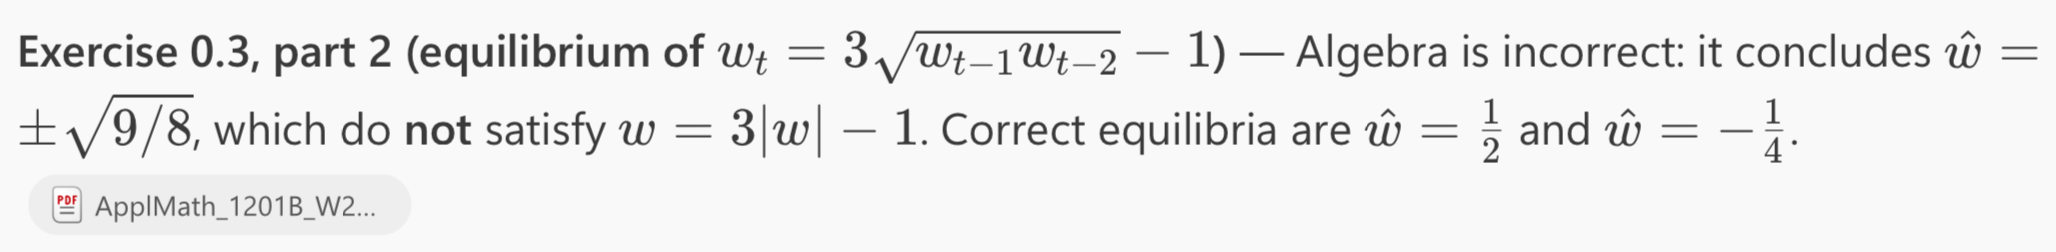
\includegraphics[width=5in]{./AI_mistake_week2_3.2.png}}
        \end{center}

      \end{solution}

    \item \(p_{t} = \frac{2}{3}p_{t-1}\).

      \begin{solution}
        Let \(\hat{p}\) denote the equilibrium solution which is a constant solution to the recurrence equation.  Replace every \(p_{t}, p_{t-1}\) by \(\hat{p}\) and solve for it.  We get
        \begin{align*}
          \hat{p} &= \frac{2}{3}\hat{p} \\
          \hat{p} &= 0.
        \end{align*}
        The only equilibrium is \(\hat{p} = 0\).
      \end{solution}

    \item \(p_{t} = \frac{2}{3}p_{t-1} - \frac{1}{5}\).

      \begin{solution}
        Let \(\hat{p}\) denote the equilibrium solution which is a constant solution to the recurrence equation.  Replace every \(p_{t}, p_{t-1}\) by \(\hat{p}\) and solve for it.  We get
        \begin{align*}
          \hat{p} &= \frac{2}{3}\hat{p} - \frac{1}{5} \\
          \hat{p} &= -\frac{3}{5}.
        \end{align*}
        The only equilibrium is \(\hat{p} = -\frac{3}{5}\).
      \end{solution}

    \item \(w_{t} = w_{t-1} - \frac{1}{5}\).
      \begin{solution}
        Let \(\hat{w}\) denote the equilibrium solution which is a constant solution to the recurrence equation.  Replace every \(w_{t}, w_{t-1}\) by \(\hat{w}\) and solve for it.  We get
        \begin{align*}
          \hat{w} &= \hat{w} - \frac{1}{5} \\
          0 &= -\frac{1}{5}.
        \end{align*}
        This is not possible. Therefore, the equilibrium solution does not exist.
      \end{solution}
  \end{enumerate}

  \hlmain{\faStar{} Compare the last three parts of this exercise.  Notice that the constants in the recurrence affect the equilibrium.}
\end{exercise}

\begin{exercise}
  How is an equilibrium different from the long-term behaviour of a recurrence?

  \begin{solution}
    Let's say \(w\) is the symbol (without the subscript) of our recurrence.

    \begin{itemize}
      \item An equilibrium solution is just a constant that satisfies the recurrence. In symbolic form, an equilibrium means \(w_{0} = w_{1} = w_{2} = \cdots\). All values of \(w_{\text{something}}\) are the same.
      \item The long-term behaviour of a recurrence is the limit \(\lim_{t \to \infty} w_{t}\). To compute this limit, we need\footnote{There are other ways to do it without solving it. But that's outside the scope of this course.} to solve the recursion to turn \(w_{t}\) into a function of \(t\).
    \end{itemize}
  \end{solution}
\end{exercise}

\begin{exercise}
  Solve the following recurrence.
  \begin{enumerate}
    \item \(v_{0} = 1\) and \(v_{t} = \frac{1}{3} v_{t-1} + \frac{1}{4}\).
      \begin{solution}
        Notice that \(a = 1/3\) and \(b = 1/4\). Because \(a \ne 1\), we have an equilibrium \(\hat{v} = \frac{b}{1-a} = \frac{1/4}{2/3} = \frac{3}{8}\).  

        Depending on your preference, either pull out the formula \(v_{t} = (v_{0} - \hat{v}) a^{t} + \hat{v}\) or go through the substitution \(v_{t} = u_{t} + \hat{v}\).  Be careful with the sign here. For some people, it is slightly less error-prone to remember the substitution as 
        \[
          (\text{old variable})_{t} = (\text{new variable})_{t} + \hat{v}.
        \]

        \begin{itemize}
          \item If you straight up use the formula, then \(v_{t} = \left(1 - \frac{3}{8}\right) \left( \frac{1}{3} \right)^{t} + \frac{3}{8}\). It is prudent to check that \(v_{t}\) is indeed a solution.  The quick sanity check is to verify the value of \(v_{0}\) against the given.

          \item If you substitute \(v_{t} = u_{t} + \hat{p}\), then \(u_{t} = v_{t} - \hat{p}\). Once again, be careful with the signs. A little sign goof here will lead to getting stuck at the next step (if you go through all the little algebra steps) or a wrong final answer (if you skip the algebra steps). That also means, if you are stuck at the next step, then look for a sign goof. 

            The recurrence becomes
            \[
              u_{0} = v_{0} - \hat{p} = \left(1 - \frac{3}{8}\right), \quad\text{and}\quad u_{t} = \frac{1}{3} u_{t-1}.
            \]
            Solve this recurrence to get \(u_{t} =\left(1 - \frac{3}{8}\right) \left(\frac{1}{3}\right)^{t}\). Put back \(v_{t}\) to get \(v_{t} = \left(1 - \frac{3}{8}\right) \left( \frac{1}{3} \right)^{t} + \frac{3}{8}\). It's the same solution as above. Once again, it is prudent to check that \(v_{t}\) is indeed a solution.  The quick sanity check is to verify the value of \(v_{0}\) against the given.
        \end{itemize}

        \hlwarn{Correction: the substitution should use the equilibrium \(\hat{v}\), not \(\hat{p}\); i.e.\ \(v_{t} = u_{t} + \hat{v}\), so \(u_{0} = v_{0} - \hat{v} = 1 - \frac{3}{8}\).}
      \end{solution}

    \item \(u_{0} = 8\) and \(u_{t} = \frac{1}{2} u_{t-1}\).
      \begin{solution}
        There isn't much to do except straight up apply the formula \(u_{t} = u_{0} a^{t}\) where \(a = \frac{1}{2}\). Therefore, 
        \[
          u_{t} = 8 \left(\frac{1}{2}\right)^{t}.
        \]

      \end{solution}
    \item \(v_{0} = 8\) and \(v_{t} = \frac{1}{2} v_{t-1} + \frac{1}{2}\).
      \begin{solution}
        Notice that \(a = 1/2\) and \(b = 1/2\). Because \(a \ne 1\), we have an equilibrium \(\hat{v} = \frac{b}{1-a} = \frac{1/2}{1/2} = 1\).  Applying the formula quickly gives us the answer \(v_{t} = 7 \left(\frac{1}{2}\right)^{t} + 1\).
      \end{solution}
      
    \item \(b_{0} = 300\) and \(b_{t} = 1.2 b_{t-1} - 10\).
      \begin{solution}
        Notice that \(A = 1.2\) and \(B = -10\). Don't forget the minus sign. Because \(A \ne 1\), we have an equilibrium \(\hat{b} = \frac{B}{1-A} = \frac{-10}{-0.2} = 50\).  Applying the formula quickly gives us the answer \(b_{t} = 250 \left(1.2\right)^{t} + 50\).

        The solutions make sense if you think of the \(1.2\) as annual return on investment and the \(-10\) as annual withdrawal. Our initial investment \(300\) earns \(300 \times 20\% = 60\) interest at the end of the first year, but we only take out \(10\). So the principle grows at the end of each year.
      \end{solution}

    \item \(a_{0} = 1000\) and \(a_{t} = 1.15 a_{t-1} + 10\).
      \begin{solution}
        Applying the formula to get \(a_{t} = \left(1000 + \frac{10}{0.15}\right) \left(1.15\right)^{t} - \left( \frac{10}{0.15} \right)\).
      \end{solution}

  \end{enumerate}
\end{exercise}

\begin{exercise}
  For each recurrence below, find the unknown parameter so that the given condition is satisfied.

  \hlmain{\faStar{} Notice the idea used in all three parts is the same. Solve the recurrence (new knowledge) and do basic algebra to find the unknown (prerequisite algebra skills).}

  \begin{enumerate}
    \item \(m_{t} = 1.02 m_{t-1} + 30\) for integers \(t \ge 1\).  Find the unknown \(m_{0}\) so that \(m_{30} = 2750\).

      \begin{solution}
        We solve the recurrence (using the formula) to get \[m_{t} = (m_{0} - \hat{m})\left( 1.02 \right)^{t} + \hat{m}, \text{ where }\hat{m} = \frac{30}{1 - 1.02}.\]  Take advantage of the given \(m_{30} = 2750\) to replace the left-hand side with \(2750\) and plug in \(t = 30\) in the right-hand side. We get a \emph{relation}
        \[
          2750 = (m_{0} - \hat{m})(1.02)^{30} + \hat{m}.
        \]
        Notice the only unknown in the equation is \(m_{0}\) because \(\hat{m} = \frac{30}{1 - 1.02}\) is a constant. Isolate for \(m_{0}\) to get 
        \[
          m_{0} = \frac{2750 - \hat{m}}{(1.02)^{30}} + \hat{m} = \frac{2750 - \frac{30}{1 - 1.02}}{(1.02)^{30}} + \frac{30}{1 - 1.02}.
        \]
        Alternatively, if you don't like the long expression on the right, then you can write a ``where`` clause like this.
        \[
          m_{0} = \frac{2750 - \hat{m}}{(1.02)^{30}} + \hat{m}, \text{ where } \hat{m} = \frac{30}{1 - 1.02}.
        \]
      \end{solution}

    \item \(b_{0} = 3000\) and \(b_{t} = a b_{t-1} - 100\) for integers \(t \ge 1\).  Suppose \(b_{17} = 1000\). Express the \(a\) in a polynomial equation, so that a computer can solve for \(a\).

      \begin{solution}
        As is with the previous part, we solve the recurrence (using the formula) to get
        \[
          b_{t} = (3000 - \hat{b}) a^{t} + \hat{b}, \text{ where } \hat{b} = \frac{-100}{1 - a}.
        \]

        Take advantage of the given \(b_{17} = 1000\) to get
        \[
          1000 = (3000 - \hat{b}) a^{17} + \hat{b}.
        \]
        Because the expression for \(\hat{b}\) has \(a\) inside, we have to plug \(\hat{b}\) into the equation. Now we have
        \[
          1000 = \left(3000 - \frac{-100}{1 - a}\right) a^{17} + \frac{-100}{1 - a}.
        \]

        This expression looks painful. The good news is that the problem-solving idea hasn't changed. We isolate for the unknown \(a\). Bite the bullet and do (high school) algebra.

        Turn everything into a quotient with \(1 - a\) in the denominator.
        \[
          1000 = \frac{((1-a) 3000 + 100)a^{17} - 100}{1 - a}.
        \]
        Watch out for goofs on the left-hand side. The left-hand side should be \(1000\) because it comes from \(b_{17}\). The numbers are specifically chosen so that you have to pay attention to algebraic details. Multiply \(1-a\) over to the left-hand side to get
        \[
          1000 (1 - a) = ((1-a) 3000 + 100)a^{17} - 100.
        \]
        A bit more rearrangement give us
        \[
          -3000 a^{18} + 3100 a^{17} + 1000 a - 1100 = 0.
        \]
        This is the polynomial relation we are looking for.

        Lots software can approximate \(a\) to arbitrary precision. The point of this exercise is to show you that the we can combine the technique of solving recurrence and some basic algebra manipulations to convert a unfamiliar problem into a familiar problem. 
      \end{solution}

    \item \(p_{0} = 1\) and \(p_{t} = \frac{1}{3} p_{t-1} + c\) for integers \(t \ge 1\).  Find the unknown \(c\) so that \(p_{10} = 1.27\).

      \begin{solution}
        The unknown \(c\) lives inside a recurrence. We can solve the recurrence to reduce the complexity of this problem. 
        \[
          p_{t} = (p_{0} - \hat{p}) \left( \frac{1}{3} \right)^{t} + \hat{p}, \text{ where } \hat{p} = \frac{c}{1 - 1/3} = \frac{3c}{2}.
        \]
        Use \(p_{10} = 1.27\) to get the equation 
        \[
          1.27 = \left(1 - \frac{3c}{2}\right) \left( \frac{1}{3} \right)^{10} + \frac{3c}{2}.
        \]
       Isolate for \(c\). High school algebra skills comes in handy. In conclusion, \(c = \frac{2}{3}\frac{1.27 - 3^{-10}}{1 - 3^{-10}}\).
      \end{solution}
  \end{enumerate}
\end{exercise}

\begin{exercise}
  A radioactive substance has a half-life of \(300\) years.   If the amount of substance is \(10\) grams at an initial time (say now), how many years will it take for the substance to decay to \(0.1\) grams?

  \begin{solution}
    For this problem, we have to be a bit careful with how we measure time. It is less error-prone to measure time in half-lives (multiples of \(300\) years). 

    Let \(m_{n}\) denote the mass of the substance in \(n\) half-life.  For example, \(m_{0}\) is its initial mass, \(m_{1}\) is its mass \(1 \times 300\) years later, \(m_{2}\) is the mass \(2 \times 300\) years later, and so on.  We have a model
    \[
      m_{0} = 10 \text{ (grams), } \text{ and } m_{n} = \frac{1}{2} m_{n-1} \text{ (grams) for \(n \ge 1\).}
    \]
    Solving this recurrence, we get
    \[
      m_{n} = 10 \left( \frac{1}{2} \right)^{n}, \text{ for } n \ge 1.
    \]

    The question translates to solving for \(n\) given \(m_{n} = 0.1\), which means we are going to solve for \(n\) given \(10 \left( \frac{1}{2} \right)^{n} = 0.1\).  A little bit of Calc~1000A manipulation later, we get \(n = \log_{2}(100) \approx 6.643\).

    In conclusion, the substance will decay to \(0.1\) gram in \(6.643\) half-lives. 

    If using half-life as a unit sounds unfamiliar (or maybe your scientific community wants everything expressed in years), then we do a little unit conversion using that \(1\) half-life is \(300\) years.  In conclusion, the substance will decay to \(0.1\) gram in
    \[
      t = 300 \; \frac{\text{years}}{\text{half-life}} \times \log_{2}(100)\; \text{half-lives} \approx 1993 \text{ years}.
    \]

  \end{solution}
\end{exercise}

\begin{exercise}
  Carbon-14 has a half-life of \(5,730\) years. If an artifact has \(7\) grams of Carbon-14 initially and has \(5\) grams left, estimate the age of the artifact.

  \begin{solution}
    As is with the previous exercise, we measure time in half-lives (multiples of \(5,730\) years). The two exercises are actually identical in spirit.

    Let \(C_{n}\) denote the mass of Carbon-14 in \(n\) half-lives.  The model is \(C_{0} = 7\) grams and \(C_{t} = \frac{1}{2}C_{n-1}\) for \(n \ge 1\), which has the solution
    \[
      C_{n} = 7 \left( \frac{1}{2} \right)^{n}, \text{ for } n \ge 1.
    \]

    The given information translates to \(C_{n} = 5\) with an unknown \(n\).  We get an equation \(5 = 7 \left( \frac{1}{2} \right)^{n}\). In conclusion, we solve for \(n\) to get
    \[
      n = \log_{2}(7/5) \text{ half-life} = 5730 \times \log_{2}(7/5) \text{ years}. 
    \]

    This is roughly \(0.4854\) half-life or, equivalently, \(2,781.5\) years.

    \hlwarn{Correction: the recurrence should read \(C_{n} = \frac{1}{2} C_{n-1}\) (subscript \(n\), not \(t\)).}
  \end{solution}
\end{exercise}

\begin{exercise}
  Suppose a person retires on January 1, 2065.

  Suppose they have one million dollars at the beginning of retirement.  The fund is invested and returns \(5\%\) interest on December 31 every year. Suppose they withdraw \(50,000\) at the beginning of each year for annual expenses, starting at retirement.

  Will this person ever run out of money? If so, when?

  \begin{solution}
    Let \(b_{t}\) denote the balance of the retirement funds on \(t\) years after January 1, 2065.  We have a model
    \[
      b_{0} = 10^{6} \text{ and } b_{t} = 1.05 b_{t-1} - 50000,\text{ for \(t \ge 1\)}.
    \]
    Solve this model, using either the formula or the substitution process, we get
    \[
      b_{t} = (b_{0} - \hat{b}) 1.05^{t} - \hat{b}, \text{ where } \hat{b} = \frac{-50000}{1 - 1.05}.
    \]

    The question asks to solve for \(t\) given \(b_{t} = 0\).  
    \begin{itemize}
      \item The \emph{mechanical} way to approach this is to pull out some algebra skills. The equation \(\left( b_{0} - \hat{b} \right) 1.05^{t} - \hat{b}\) rearranges to \(1.05^{t} = \frac{\hat{b}}{b_{0} - \hat{b}}\) which is solved by
        \[
          t = \log_{1.05}\left( \frac{\hat{b}}{b_{0} - \hat{b}} \right) \overset{\text{plug in numbers}}{=} \log_{1.05}\left( \frac{\hat{b}}{{\color{warn} 0}} \right)?!?!
        \]
        The equation says \(t\) cannot be found. It does not mean we have failed. We just need a bit of reality check.  Notice that \(\hat{b} = 10^{6}\). The person's initial fund is exactly the equilibrium solution, which means the balance \(b_{t}\) never changes. In conclusion, this person will never run out of money. 

        Nice. A million dollars was seen as a golden number 30 years ago. Heard of the song \emph{If I had a million dollars} by Barenaked Ladies?

      \item We could have started with a little calculation to pick up some intuition. Let's straight up calculate \(b_{1}, b_{2}, b_{3}\) using the recursion to get
        \[
          b_{1} = 10^{6}, b_{2} = 10^{6}, b_{3} = 10^{6}.
        \]
        We \emph{suspect} that the balance does not change which means the initial fund is probably just the equilibrium.  Verify this by showing \(\hat{b} = 10^{6}\). We can now conclude that the person will never run out of money.
    \end{itemize}

    Don't be fooled that the shorter approach is always better. Let's say we change the withdrawal amount to be \(49,000\) per year. Then you can verify that the initial investment is NOT the equilibrium solution. In such a case, we probably suspect that the balance grows unbounded and need to show by a precise calculation that \(\lim_{t \to \infty} b_{t} = \infty\). We would need to solve the recursion and do a little calculus, which is (slightly) faster had one simply started with the first approach.

    \hlwarn{Correction: the general solution should read \(b_{t} = (b_{0} - \hat{b})\,1.05^{t} + \hat{b}\) (with \(+\hat{b}\)). It happens not to affect the conclusion here because \(b_{0} = \hat{b} = 10^{6}\).}
  \end{solution}
\end{exercise}

\begin{exercise}
  Someone plans to retire on January 1 some time in the future.

  Suppose their expenses is \(80,000\) per year withdrawn at the beginning of each year from their retirement fund. Moreover, suppose the retirement fund is invested and returns \(7\%\) interest on December 31 every year. 

  What is the minimum amount of money needed at the beginning of the retirement if the person is expected to live \(25\) years in the retirement?

  \begin{solution}
    Let \(b_{t}\) denote the balance of the retirement funds on \(t\) years after January 1, some year in the future.  We have a model 
    \[
      b_{0} \text{ is unknown}  \text{ and } b_{t} = 1.07 b_{t-1} - 80000,\text{ for \(t \ge 1\)}.
    \]
    Solve this model, using either the formula or the substitution process, we get
    \[
      b_{t} = (b_{0} - \hat{b}) 1.07^{t} - \hat{b}, \text{ where } \hat{b} = \frac{-80000}{1 - 1.07}.
    \]

    It is easier to solve for \(b_{0}\) given \(b_{25} = 0\). There is no shortcut in this case. We start with the equation
    \[
      0 = (b_{0} - \hat{b}) 1.07^{25} + \hat{b}.
    \]
    Isolate for \(b_{0}\) to get 
    \[
      b_{0} = \frac{-\hat{b} + \hat{b} 1.07^{25}}{1.07^{25}} \approx 932,230.
    \]

    In conclusion, one needs \emph{at least} \(\$ 932,230\) to have enough money for retirement in this scenario.

    \hlwarn{Correction: the general solution line should read \(b_{t} = (b_{0} - \hat{b})\,1.07^{t} + \hat{b}\) (with \(+\hat{b}\), as already used in the next line). Also, the numerical value is \(b_{0} \approx 932{,}286\), not \(932{,}230\).}
  \end{solution}
\end{exercise}
\end{document}
